%Version 3 October 2023
% See section 11 of the User Manual for version history
%
%%%%%%%%%%%%%%%%%%%%%%%%%%%%%%%%%%%%%%%%%%%%%%%%%%%%%%%%%%%%%%%%%%%%%%
%%                                                                 %%
%% Please do not use \input{...} to include other tex files.       %%
%% Submit your LaTeX manuscript as one .tex document.              %%
%%                                                                 %%
%% All additional figures and files should be attached             %%
%% separately and not embedded in the \TeX\ document itself.       %%
%%                                                                 %%
%%%%%%%%%%%%%%%%%%%%%%%%%%%%%%%%%%%%%%%%%%%%%%%%%%%%%%%%%%%%%%%%%%%%%

%%\documentclass[referee,sn-basic]{sn-jnl}% referee option is meant for double line spacing

%%=======================================================%%
%% to print line numbers in the margin use lineno option %%
%%=======================================================%%

%%\documentclass[lineno,sn-basic]{sn-jnl}% Basic Springer Nature Reference Style/Chemistry Reference Style

%%======================================================%%
%% to compile with pdflatex/xelatex use pdflatex option %%
%%======================================================%%


\documentclass[sn-mathphys-ay, Numbered]{sn-jnl}

%%%% Standard Packages
%%<additional latex packages if required can be included here>

\usepackage{graphicx}%
\usepackage{caption}
\usepackage{multirow}%
\usepackage{subcaption}
\usepackage{amsmath,amssymb,amsfonts}%
\usepackage{amsthm}%
\usepackage{mathrsfs}%
\usepackage[title]{appendix}%
\usepackage{xcolor}%
\usepackage{textcomp}%
\usepackage{manyfoot}%
\usepackage{booktabs}%
\usepackage{algorithm}%
\usepackage{algorithmicx}%
\usepackage{algpseudocode}%
\usepackage{listings}%

\usepackage{tikz}
\usetikzlibrary{positioning}

%%%%
\usepackage{natbib}
% \bibliographystyle{sn-basic}

%%%%%=============================================================================%%%%
%%%%  Remarks: This template is provided to aid authors with the preparation
%%%%  of original research articles intended for submission to journals published 
%%%%  by Springer Nature. The guidance has been prepared in partnership with 
%%%%  production teams to conform to Springer Nature technical requirements. 
%%%%  Editorial and presentation requirements differ among journal portfolios and 
%%%%  research disciplines. You may find sections in this template are irrelevant 
%%%%  to your work and are empowered to omit any such section if allowed by the 
%%%%  journal you intend to submit to. The submission guidelines and policies 
%%%%  of the journal take precedence. A detailed User Manual is available in the 
%%%%  template package for technical guidance.
%%%%%=============================================================================%%%%

%% as per the requirement new theorem styles can be included as shown below
\theoremstyle{thmstyleone}%
\newtheorem{theorem}{Theorem}%  meant for continuous numbers
%%\newtheorem{theorem}{Theorem}[section]% meant for sectionwise numbers
%% optional argument [theorem] produces theorem numbering sequence instead of independent numbers for Proposition
\newtheorem{proposition}[theorem]{Proposition}% 
%%\newtheorem{proposition}{Proposition}% to get separate numbers for theorem and proposition etc.

\theoremstyle{thmstyletwo}%
\newtheorem{example}{Example}%
\newtheorem{remark}{Remark}%

\theoremstyle{thmstylethree}%
\newtheorem{definition}{Definition}%

\raggedbottom
%\unnumbered% uncomment this for unnumbered level heads
\geometry{bottom=1.6in}

\begin{document}

\title[Leveraging LSTM and Attention Mechanisms for Improved Fake News Detection]{Leveraging LSTM and Attention Mechanisms for Improved Fake News Detection}

%%=============================================================%%
%% GivenName	-> \fnm{Joergen W.}
%% Particle	-> \spfx{van der} -> surname prefix
%% FamilyName	-> \sur{Ploeg}
%% Suffix	-> \sfx{IV}
%% \author*[1,2]{\fnm{Joergen W.} \spfx{van der} \sur{Ploeg} 
%%  \sfx{IV}}\email{iauthor@gmail.com}
%%=============================================================%%

\author*[1]{\fnm{Nicolò} \sur{Rosati}}\email{nicolo.rosati@studenti.unimi.it}


\affil*[1]{\orgdiv{Department of Computer Science}, \orgname{Università degli Studi di Milano}, \orgaddress{\street{Via Celoria 18}, \city{Milano}, \postcode{20133}}}


%%==================================%%
%% Sample for unstructured abstract %%
%%==================================%%

\abstract{The explosion of digital media has transformed information sharing, connecting people worldwide and accelerating news dissemination. This rapid spread, however, has also fueled the proliferation of fake news—false or misleading information disguised as legitimate reporting. The consequences are significant, impacting public opinion, damaging public trust, and threatening democratic processes.
	
Combating fake news requires innovative solutions that go beyond traditional fact-checking, which is often slow and struggles to keep up with the rapid spread of misinformation. To address this, a machine learning framework has been developed to automatically classify news articles as true or false. This approach utilizes natural language processing (NLP) and advanced neural networks. Key components include thorough data preprocessing, extracting meaningful features using word embeddings, and employing Long Short-Term Memory (LSTM) networks enhanced with attention mechanisms. By addressing each critical stage of fake news detection, this methodology aims to provide a scalable and robust solution to this pressing digital-age problem.}

\maketitle

\section{Introduction}\label{sec1}

The dissemination of fake news has become a pressing issue with far-reaching consequences, influencing political decisions, public health initiatives, and societal trust on a global scale \citep{Lazer_2018}. The rapid growth of digital platforms has made it easier than ever to share information, but it has also created fertile ground for the spread of misinformation. Traditional methods of fact-checking, while effective, are labour-intensive and unable to match the pace at which fake news proliferates online.

The advent of machine learning provides a powerful alternative by enabling the automatic classification of news articles based on their truthfulness. Unlike manual efforts, machine learning models can process vast amounts of textual data in real time, making them highly suitable for combating the dynamic and evolving nature of misinformation. In this project, a deep learning-based hybrid framework is proposed, which utilises Word2Vec embeddings and Long Short-Term Memory (LSTM) networks enhanced by attention for fake news detection. As part of this approach, Word2Vec embeddings are generated to obtain vector representations of news excerpts. These embeddings play a crucial role in producing context-free and data-agnostic feature vectors, effectively capturing semantic and syntactic relationships in the text.

\section{Related Work}\label{sec2}

Fake news detection has become a crucial research area due to its impact on societal trust, politics, and public health. Over time, various methods have been developed, each with strengths and limitations.

Early approaches focused on lexical analysis, examining linguistic patterns like word frequency and sentiment. While useful for identifying stylistic differences, they struggled with semantic meaning and context \citep{Perez-Rosas2017}. Machine learning methods, such as Support Vector Machines (SVMs), Random Forests, and Logistic Regression, improved classification but required extensive feature engineering and faced challenges with textual variability.

The rise of deep learning transformed fake news detection. Models like Convolutional Neural Networks (CNNs) and Long Short-Term Memory (LSTM) networks have been widely adopted—CNNs excel at recognizing local patterns, while LSTMs capture long-range dependencies, making them effective for sequential text analysis. Hybrid approaches further enhanced performance by integrating linguistic features with network analysis or external knowledge base \citep{Shu2019}.

Despite progress, challenges remain, including linguistic diversity, satire, and evolving misinformation tactics. Many models also struggle with generalizability across domains \citep{Lit_Rev}.

This project adopts a hybrid framework combining advanced text preprocessing, Word2Vec embeddings, and LSTM networks with attention mechanisms. By leveraging these techniques, it aims to address previous limitations and enhance fake news detection.

\section{Dataset Preparation}
Preparing the dataset is a crucial first step in developing an effective fake news detection system. The dataset began with 71,406 news articles, balanced at 51\% true and 49\% fake. Each entry in the dataset included a news title, news text, and a label (1 for fake and 0 for true). Addressing quality issues required overcoming multiple challenges through a series of targeted steps.
\subsection{Removal of Non-English Articles}
Non-English articles were identified and removed from the dataset to ensure linguistic uniformity. A total of 1,355 such articles were found and excluded. Mixing languages could introduce noise and hinder the model's ability to capture language-specific nuances critical for accurate detection. By retaining only English-language articles, the dataset was streamlined for a more focused analysis, eliminating potential variability in syntactic and semantic structures caused by multilingual content.

\subsection{Elimination of Duplicate Entries}
Duplicate articles were identified and removed, resulting in the exclusion of 8,132 duplicates from the dataset. Such duplicates have the potential to distort the dataset by disproportionately representing certain patterns, thereby introducing bias into the model’s learning process.

\subsection{Final Dataset}
Following the dataset preparation process, the final state of the dataset reflects substantial improvements in quality and relevance. 

The final dataset consists of 61,919 English-language news articles, with a distribution of 56\% true and 44\% fake news. This near balance ensures that the model is trained on a dataset that fairly represents both classes, minimizing the risk of bias in classification. To have a clear view of the dataset, Figure \ref{fig:wordclouds} illustrates the Word Cloud representation for each class.
\begin{figure}[t]
	\makebox[\textwidth][c]{
		\begin{minipage}{1.2\textwidth}
			\begin{subfigure}
				{0.65\textwidth} \hspace{-1.2cm}
				\includegraphics[width=0.90\linewidth]{images/wordCloudTrue.png}
				\caption{\hspace{3.5 cm} \phantom{.}}
				\label{fig:first}
			\end{subfigure}
			% \hfill
            \hspace{-.3cm}
			\begin{subfigure}
				{0.65\textwidth} \hspace{-1.7cm}
				\includegraphics[width=0.90\linewidth]{images/wordCloudFalse.png}
				\caption{\hspace{4 cm} \phantom{.}}
				\label{fig:second}
			\end{subfigure}
		\end{minipage}
	}
	\caption{Word cloud representations of the dataset: (a) for real news, (b) for fake news.}
	\label{fig:wordclouds}
\end{figure}

\section{Text Preprocessing}
This chapter describes the text preprocessing procedures applied to the raw data in this project. Preprocessing is a fundamental step in NLP tasks, converting raw text into a format that can be effectively utilised by machine learning models. The pipeline used in this project is designed to clean, normalise, and extract meaningful features from the text, with the ultimate goal of improving the model's performance in detecting fake news.

\subsection{Cleaning and Lowercasing}
The first step in preprocessing involves cleaning the text. This includes removing irrelevant elements such as punctuation, symbols, and numerical digits, which do not contribute to textual meaning. Additionally, all text is converted to lowercase to ensure consistency and minimize the impact of case variations on the model's performance. The news title and text were then merged together to form a single input, allowing the model to consider both components as a cohesive piece of information.

\subsection{Tokenisation and Stopword Removal}
After cleaning, the text is broken down into smaller units, or tokens, through a process called tokenisation. However, not all tokens are equally informative. Common words like "the," "a," and "is" (referred to as stop words) often add little value to the meaning of a sentence. These stop words are removed to allow the model to focus on content-rich words that are more likely to indicate whether a news article is genuine or fabricated.

\subsection{Lemmatisation}
Words often appear in various grammatical forms depending on their context. For instance, the word "run" can take forms like "running" or "runs." While these variations may differ slightly in meaning, they share a common root. Lemmatisation reduces words to their base form, or lemma, ensuring that semantic similarities are captured while reducing the number of unique words the model needs to process.

In this project, the WordNet library is used for lemmatisation. WordNet maps words to their corresponding lemmas by considering their part-of-speech (POS) tags. By incorporating POS tagging, the process ensures that each word's lemma is selected accurately based on its grammatical context.

\subsection{The Preprocessing Pipeline}
The individual steps described above are combined into a cohesive preprocessing pipeline to streamline text processing. The pipeline takes raw text data as input and outputs preprocessed text, which is then fed into the fake news detection model.

By integrating cleaning, tokenisation, stopword removal, and lemmatisation, the pipeline extracts the most relevant features from the text. This helps the machine learning model focus on the critical content, ultimately improving its ability to distinguish between authentic and fake news. Figure \ref{fig:preprocessing-pipeline} shows an example of the final preprocessing pipeline.

\begin{figure}[H]
	\centering
	% \vspace*{0.5cm}
	\scalebox{0.65}{ % Adjust scale to fit the page
		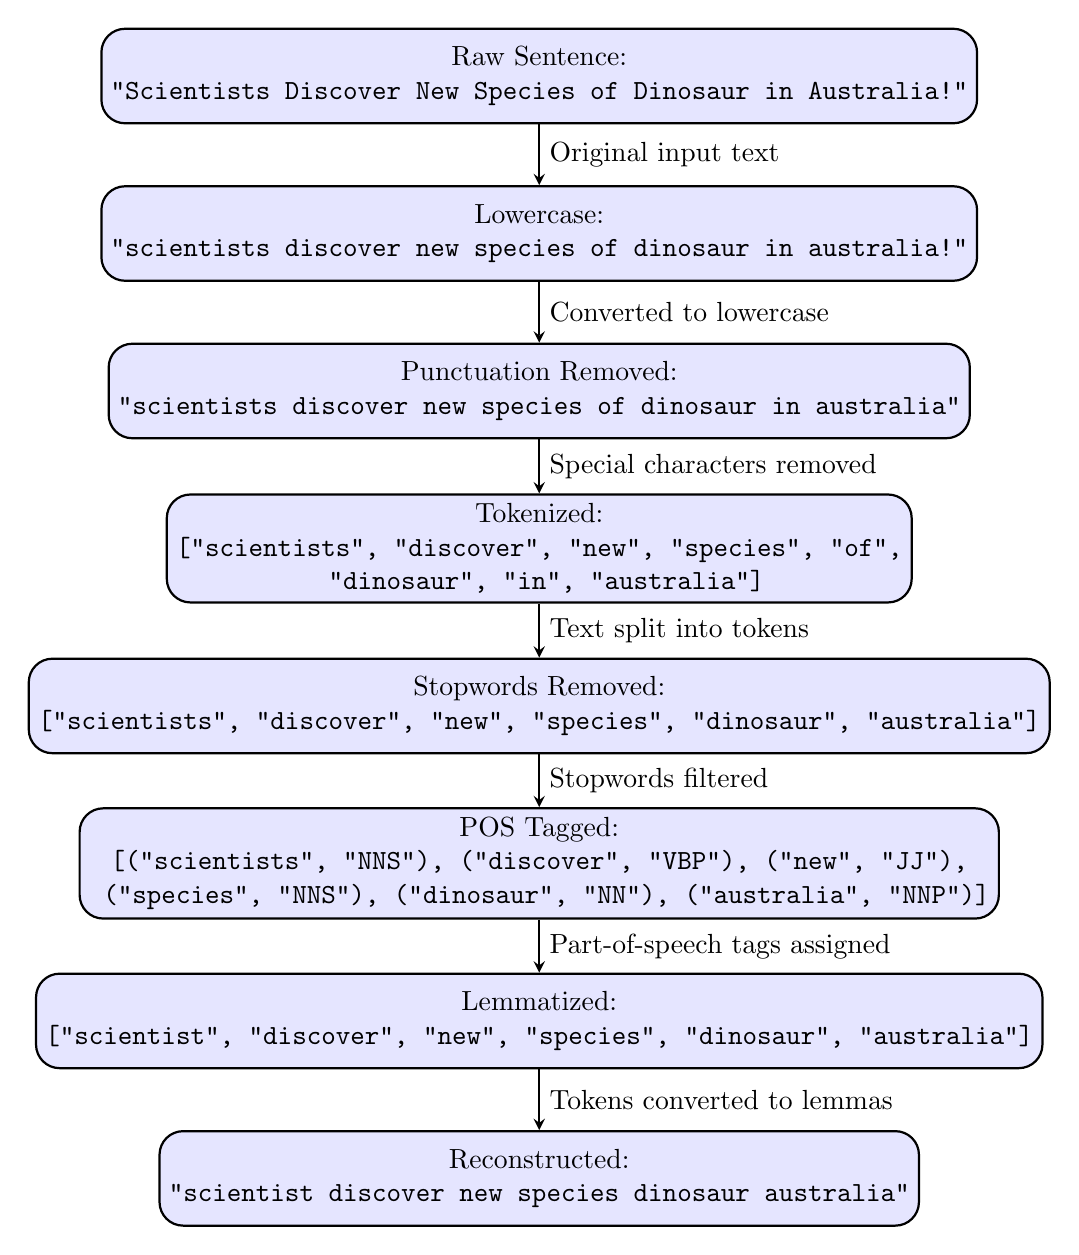
\begin{tikzpicture}[
				node distance=1.4cm,
				box/.style={
					rectangle,
					draw=black,
					thick,
					minimum width=7cm,
					minimum height=1.2cm,
					align=center,
					rounded corners=3mm,
					fill=blue!10
				},
				arrow/.style={
					->,
					thick,
					>=stealth
				}
			]
			% Nodes
			\node[box] (raw) at (0,0) {Raw Sentence:\\ \texttt{"Scientists Discover New Species of Dinosaur in Australia!"}};
			        
			\node[box] (lowercase) at (0,-2) {Lowercase:\\ \texttt{"scientists discover new species of dinosaur in australia!"}};
			\node[box] (punctuation) at (0,-4) {Punctuation Removed:\\ \texttt{"scientists discover new species of dinosaur in australia"}};
			\node[box] (tokenization) at (0,-6) {Tokenized: \\ \texttt{["scientists", "discover", "new", "species", "of",}\\ \texttt{ "dinosaur", "in", "australia"]}};
			\node[box] (stopwords) at (0,-8) {Stopwords Removed:\\ \texttt{["scientists", "discover", "new", "species", "dinosaur", "australia"]}};
			\node[box] (pos) at (0,-10) {POS Tagged:\\ \texttt{[("scientists", "NNS"), ("discover", "VBP"), ("new", "JJ"),}\\ \texttt{ ("species", "NNS"), ("dinosaur", "NN"), ("australia", "NNP")]}};
			\node[box] (lemmatization) at (0,-12) {Lemmatized:\\ \texttt{["scientist", "discover", "new", "species", "dinosaur", "australia"]}};
			\node[box] (reconstruction) at (0,-14) {Reconstructed:\\ \texttt{"scientist discover new species dinosaur australia"}};
			        
			\draw[arrow] (raw) -- (lowercase) node[midway,right] {Original input text};
			\draw[arrow] (lowercase) -- (punctuation) node[midway,right] {Converted to lowercase};
			\draw[arrow] (punctuation) -- (tokenization) node[midway,right] {Special characters removed};
			\draw[arrow] (tokenization) -- (stopwords) node[midway,right] {Text split into tokens};
			\draw[arrow] (stopwords) -- (pos) node[midway,right] {Stopwords filtered};
			\draw[arrow] (pos) -- (lemmatization) node[midway,right] {Part-of-speech tags assigned};
			\draw[arrow] (lemmatization) -- (reconstruction) node[midway,right] {Tokens converted to lemmas};
		\end{tikzpicture}}
	\caption{Text Preprocessing Pipeline}
	\label{fig:preprocessing-pipeline}
\end{figure}
\section{Word Embedding}
Word embeddings are fundamental in natural language processing for representing textual data in a semantically and syntactically meaningful way \citep{embeddingsClose, Jurafsky2019Speech}. This project employed pre-trained Word2Vec embeddings using the Continuous Bag-of-Words (CBOW) approach due to their established effectiveness in capturing rich contextual information about words \citep{word2VecEfficient}.

Word embeddings map words to dense, fixed-length vectors in a continuous vector space. This contrasts with traditional one-hot encoding, which produces sparse, high-dimensional representations that fail to capture semantic relationships. Word embeddings, conversely, encode nuanced relationships between words. For instance, semantically similar words like 'fake' and 'misleading' are located closer together in the embedding space, reflecting their shared meaning \citep{embeddingsClose}.

Utilizing pre-trained Word2Vec embeddings offered several key advantages. Firstly, these embeddings are trained on massive text corpora, enabling the model to leverage knowledge far exceeding the available training dataset \citep{levy-etal-2015-improving}. This is particularly beneficial when dealing with limited dataset sizes. Secondly, pre-trained embeddings drastically reduce computational costs by utilizing existing representations instead of training them from scratch \citep{PreTrainEmb}. This transfer learning approach allows for faster training and often improved performance, especially with limited data.

To ensure consistent input dimensions for the model, input sequences were padded or truncated to a fixed length. Padding involved adding zero vectors to shorter sequences, while truncation shortened longer sequences to the predetermined length. This preprocessing step is crucial because neural networks require fixed-size input vectors to operate effectively.

By leveraging word embeddings, the model was equipped with a powerful mechanism to understand and exploit inter-word relationships. This capability allowed the model to identify subtle linguistic cues differentiating fake news from genuine news, ultimately contributing to improved accuracy and robustness of the fake news detection system \citep{rashkin-etal-2017-truth}.

\section{Model Architecture}\label{sec:Models}
In this project, two different models were evaluated: an LSTM model and an LSTM with attention model.

\subsection{Long Short-Term Memory Networks}

Long Short-Term Memory (LSTM) networks represent an advanced class of Recurrent Neural Networks (RNNs) specifically designed to address the limitations associated with modeling long-range dependencies in sequential data. Traditional RNNs are inherently limited by the vanishing gradient problem \citep{LSTM}, which restricts their capacity to capture dependencies spanning long sequences. This limitation is particularly problematic in natural language processing tasks, where capturing the contextual nuances of text is critical—especially in applications such as misinformation detection.

At the core of the LSTM architecture lies the cell state, denoted as \( c_t \), which serves as a memory unit that propagates relevant information through time. To regulate the flow of information, the LSTM utilizes three primary gating mechanisms: the forget gate, the input gate, and the output gate.

\subsubsection{Forget Gate}
The forget gate is responsible for determining which portions of the previous cell state \( c_{t-1} \) should be discarded. This is achieved by computing a gating vector \( f_t \) based on the previous hidden state \( h_{t-1} \) and the current input \( x_t \):
\[
f_t = \sigma\!\left(W_f \cdot \begin{bmatrix} h_{t-1} \\ x_t \end{bmatrix} + b_f\right)
\]
Here, \( W_f \) is the weight matrix, \( b_f \) is the bias vector, and \( \sigma \) represents the logistic sigmoid activation function. The elements of \( f_t \) lie between 0 and 1, with values closer to 0 indicating that the corresponding information in \( c_{t-1} \) should be forgotten, and values closer to 1 indicating retention.

\subsubsection{Input Gate}
The input gate regulates the incorporation of new information into the cell state. It consists of two parts. First, a candidate vector \( \tilde{c}_t \) is computed:
\[
\tilde{c}_t = \tanh\!\left(W_c \cdot \begin{bmatrix} h_{t-1} \\ x_t \end{bmatrix} + b_c\right)
\]
Simultaneously, an input modulation vector \( i_t \) is obtained:
\[
i_t = \sigma\!\left(W_i \cdot \begin{bmatrix} h_{t-1} \\ x_t \end{bmatrix} + b_i\right)
\]
The cell state is then updated by combining the scaled previous cell state with the new candidate information:
\[
c_t = f_t \odot c_{t-1} + i_t \odot \tilde{c}_t
\]
In this equation, \( \odot \) denotes element-wise multiplication.

\subsubsection{Output Gate}
The output gate controls the flow of information from the cell state to the hidden state \( h_t \), which is subsequently passed on to future layers or time steps. The output gate computes a gating vector \( o_t \):
\[
o_t = \sigma\!\left(W_o \cdot \begin{bmatrix} h_{t-1} \\ x_t \end{bmatrix} + b_o\right)
\]
The new hidden state is then derived by applying the hyperbolic tangent function to the cell state and modulating it with \( o_t \):
\[
h_t = o_t \odot \tanh(c_t)
\]

This intricate gating mechanism enables LSTMs to effectively mitigate the vanishing gradient problem by selectively retaining or discarding information. Consequently, LSTMs are well-equipped to model long-range dependencies in sequential data, which is essential for capturing the complex linguistic structures inherent in natural language processing tasks.


\subsection{Attention Mechanism}

While LSTMs effectively process sequential information, they may not always focus on the most crucial aspects of the input text. This limitation can be addressed by incorporating an attention mechanism \citep{Attention}. The attention mechanism dynamically assigns weights to different parts of the input sequence, thereby enabling the model to concentrate on the segments that are most relevant for a given prediction.

Assume that an LSTM processes an input sequence and produces a series of hidden states \(\{h_1, h_2, \ldots, h_T\}\), where \(T\) is the length of the sequence. The attention mechanism computes a score \(e_i\) for each hidden state \(h_i\) to evaluate its importance relative to the current prediction. 
\clearpage
One common formulation is:

\[
e_i = \mathbf{v}^T \tanh(W_h h_i + W_s s),
\]

where:
\begin{itemize}
    \item \(W_h\) and \(W_s\) are learnable weight matrices,
    \item \(s\) is a context vector (which could be the current state of a decoder or a query vector in other attention paradigms),
    \item \(\mathbf{v}\) is a learnable parameter vector,
    \item and \(\tanh\) is the hyperbolic tangent activation function.
\end{itemize}

These scores \(e_i\) are normalized using the softmax function to yield the attention weights \(\alpha_i\):

\[
\alpha_i = \frac{\exp(e_i)}{\sum_{j=1}^{T} \exp(e_j)}.
\]

The weights \(\alpha_i\) indicate the relative importance of each hidden state in the context of the current prediction. Using these weights, a context vector \(c\) is computed as a weighted sum of the hidden states:

\[
c = \sum_{i=1}^{T} \alpha_i h_i.
\]

This context vector \(c\) is then combined with other relevant vectors (for example, the state \(s\)) to produce the final prediction. In effect, the attention mechanism allows the model to dynamically adjust its focus by emphasizing important words or phrases and diminishing the influence of less relevant information.

More specifically, the attention mechanism enhances the model's capabilities in two key ways:

\begin{itemize}
    \item \textbf{Identify Key Indicators:} By assigning higher weights to critical words or phrases (such as those with exaggerated claims like ``groundbreaking discovery'' or emotionally charged terms like ``crisis''), the attention mechanism enables the model to focus on specific indicators that strongly suggest fake news.
    
    \item \textbf{Improve Interpretability:} The distribution of attention weights offers insights into the model's decision-making process by highlighting which parts of the text contributed most significantly to the prediction. This transparency is especially valuable for understanding the factors that lead to the classification of a news article as fake or real.
\end{itemize}

Through these mechanisms, the attention module provides a powerful means to enhance both the performance and interpretability of models dealing with complex sequential data, such as those used in fake news detection.

\subsection{Hyperparameters tuning}
The selected hyperparameters were determined through experimentation and were found to yield the best classification results across the two models. Both models utilise a dropout rate of 0.4. The AdamW optimizer is used, and the loss function is BCEWithLogitsLoss, appropriate for binary classification tasks. The final output layer employs a Sigmoid activation function. Training was conducted for 10 epochs, as the training loss stabilized after this duration, with a batch size of 64. An early stopping mechanism was applied to prevent overfitting, and the ReduceLROnPlateau scheduler adjusts the learning rate when validation accuracy ceases to improve. For the ReduceLROnPlateau scheduler, an initial learning rate of 0.00005 was set, with a reduction factor of 0.25 and a patience of 3 epochs.

The Word2Vec embedding dimension is set to 300, with input text truncated to 623 tokens, corresponding to the 90th percentile of text lengths in the dataset.
\section{Results and Analysis}
\subsection{Overall performance}
The LSTM model with an attention mechanism consistently outperforms the standard LSTM across all key metrics. The incorporation of attention significantly enhances both model accuracy and stability during training, leading to more reliable predictions and improved generalisation.
\subsection{Training dynamics}
Analysis of the accuracy curves (Figure \ref{fig:acc_comp}) reveals that the attention-based model exhibits rapid initial learning and attains higher performance levels earlier in the training process. Specifically, it achieves approximately 90\% accuracy by epoch 2, whereas the standard LSTM model requires up to epoch 4 to reach 80\% accuracy. Moreover, the attention model demonstrates greater stability throughout training, while the standard LSTM exhibits considerable volatility, particularly in the validation metrics.

\subsection{ROC and AUC Analysis}
The Receiver Operating Characteristic (ROC) (Figure \ref{fig:roc_comp}) curves highlight a substantial difference in the discriminative ability of the models. The attention-based model achieves an Area Under the Curve (AUC) of 0.995, compared to 0.879 for the standard LSTM. This substantial gap indicates that the attention-enhanced model is significantly better at distinguishing between classes across different classification thresholds. Furthermore, the steeper ROC curve of the attention model suggests higher true positive rates while maintaining lower false positive rates.

\subsection{F1 Score Performance}
The F1 score analysis (Figure \ref{fig:f1_comp}) indicates that the attention model maintains consistently higher and more stable performance, with scores exceeding 0.90 across epochs. Conversely, the standard LSTM fluctuates around 0.80, reflecting a weaker balance between precision and recall. This stability further reinforces the advantages of incorporating an attention mechanism.

\subsection{Loss Patterns}
The loss curves (Figure \ref{fig:loss_comp}) demonstrate that the attention-based model consistently achieves lower training and validation loss values throughout the training process. It exhibits more efficient learning, characterised by a steeper initial descent and convergence to a more optimal minimum. In contrast, the standard LSTM model maintains higher loss values and displays greater instability, indicating less effective learning dynamics.

\subsection{Confusion Matrix Analysis}
The confusion matrices provide further insights into classification performance. The attention-based model, as shown in Figure  \ref{fig:conf_att} and Figure \ref{fig:conf_no_att} achieves a better-balanced classification with:
\begin{itemize}
	\item A higher true negative rate (6,677 vs. 6,298)
	\item Fewer false positives (270 vs. 9649)
	\item More accurately classified positive cases (5,258 vs. 4,089 true positives)
	\item A lower false negative rate (179 vs. 1,350)
\end{itemize}
These improvements suggest that the attention mechanism enhances both sensitivity and specificity, reducing the likelihood of both false positives and false negatives.
\subsection{Precision-Recall Characteristics}
The precision-recall curves (Figure \ref{fig:prec_rec_comp}) further underscore the superiority of the attention mechanism. The attention-based model maintains high precision even at elevated recall values, achieving an AUC of 0.9993, whereas the standard LSTM’s performance degrades more rapidly (AUC = 0.830). This suggests that the attention mechanism enhances reliability in positive predictions and achieves a superior balance between precision and recall.
\subsection{Precision Analysis}
Precision metrics further highlight the advantages of the attention mechanism. The attention-based model consistently achieves precision values above 0.90, whereas the standard LSTM’s fluctuates between 0.75 and 0.85. The ability of the attention mechanism to sustain high precision, even as recall improves, suggests an overall enhancement in discriminatory performance.
\subsection{Recall Analysis}
Recall metrics reveal that the attention-based model consistently achieves recall values around 0.95. In contrast, the standard LSTM model shows greater variability, with recall values oscillating between 0.70 and 0.90. The stability and high recall observed in Model 1 further underscore the benefits conferred by the attention mechanism.


\subsection{Practical Implications}
The attention mechanism delivers substantial benefits for this classification task. Beyond improving overall performance metrics, it enhances prediction stability and reliability. The reduction in false positives and false negatives is particularly valuable in applications where misclassification costs are high. Additionally, faster convergence and increased training stability make the model more practical for real-world deployment, ensuring consistent performance under various conditions.

\section{Conclusion}
The integration of an attention mechanism significantly enhances the LSTM model’s performance across all evaluated dimensions, from raw accuracy to nuanced metrics such as precision-recall balance and classification stability. The empirical evidence strongly supports the use of attention-based LSTMs for this application, as they yield superior absolute performance and more robust learning characteristics.

\begin{figure}[H]
	\vspace{-1cm}
	\makebox[\textwidth][c]{
		\begin{minipage}{1.5\textwidth}
			\centering
			% First row
			\begin{subfigure}[b]{0.40\textwidth}
				\includegraphics[width=\textwidth]{images/accuracy_comparison.png}
				\caption{Accuracy Comparison}
                \label{fig:acc_comp}
			\end{subfigure}%
			\begin{subfigure}[b]{0.40\textwidth}
				\includegraphics[width=\textwidth]{images/auc_roc_curve_comparison.png}
				\caption{ROC Curve Comparison}
                \label{fig:roc_comp}
			\end{subfigure}%
			        
			        
			\vspace{1em}
            \begin{subfigure}[b]{0.40\textwidth}
				\includegraphics[width=\textwidth]{images/f1_score_comparison.png}
				\caption{F1 Score Comparison}
                \label{fig:f1_comp}
			\end{subfigure}%
			\begin{subfigure}[b]{0.40\textwidth}
				\includegraphics[width=\textwidth]{images/loss_comparison.png}
				\caption{Loss Comparison}
                \label{fig:loss_comp}
			\end{subfigure}
			\vspace{1em}
			
			        
			\begin{subfigure}[b]{0.40\textwidth}
				\includegraphics[width=\textwidth]{images/confusion_matrix_comparison_Model_1.png}
				\caption{LSTM with Attention Confusion Matrix}
                \label{fig:conf_att}
			\end{subfigure}%
			\begin{subfigure}[b]{0.40\textwidth}
				\includegraphics[width=\textwidth]{images/confusion_matrix_comparison_Model_2.png}
				\caption{LSTM without Attention Confusion Matrix}
                \label{fig:conf_no_att}
			\end{subfigure}
			\caption{Model Performance Comparisons}
			\label{fig:model_comparisons}
		\end{minipage}
	}
\end{figure}


\begin{figure}[H]
	\makebox[\textwidth][c]{
		\begin{minipage}{1.5\textwidth}
			\centering
			\vspace{1em}
            \begin{subfigure}[b]{0.40\textwidth}
				\includegraphics[width=\textwidth]{images/precision_recall_curve_comparison.png}
				\caption{Precision-Recall Comparison}
                \label{fig:prec_rec_comp}
			\end{subfigure}%
			\begin{subfigure}[b]{0.40\textwidth}
				\includegraphics[width=\textwidth]{images/precision_comparison.png}
				\caption{Precision-Recall Curve}
                \label{fig:prec_comp}
			\end{subfigure}
			        
			\begin{subfigure}[b]{0.40\textwidth}
				\includegraphics[width=\textwidth]{images/recall_comparison.png}
				\caption{Recall Comparison}
                \label{fig:rec_comp}
			\end{subfigure}
			\caption{Model Performance Comparisons}
			\label{fig:model_comparisons}
		\end{minipage}
	}
\end{figure}
\bibliography{sn-bibliography}
\end{document}